\capitulo{6}{Trabajos relacionados}\label{cap:trabajosRelacionados}

Este capítulo mostrara algunos trabajos que se han hecho con sistemas empotrados. De esta manera podremos hacernos a la idea de algunas de las aplicaciones reales de estos sistemas. Veamos los distintos sectores en los que se utilizan los SE:

\section{SE en equipos médicos}\label{sec:TREquiposMedicos}

Muchos de los aparatos que se utilizan de forma periódica en la sanidad, usan un microcontrolador \cite{medicinaSE}. La Figura \ref{PresionSanguinea} muestra un ejemplo de un medidor de presión sanguínea:

%\imagen{presionSangre}{Esquema arquitectónico de un SE de medición de sangre.} \label{PresionSanguinea}
\begin{figure}[!h]
	\centering
	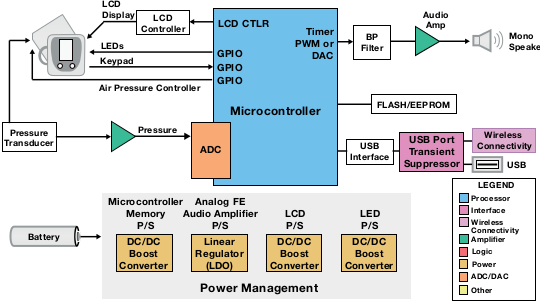
\includegraphics[width=0.9\textwidth]{presionSangre}
	\caption{Esquema arquitectónico de un SE de medición de sangre.}\label{PresionSanguinea}
\end{figure}

En la imagen podemos apreciar como existen dos partes importantes, por un lado tenemos todos los elementos que necesitan corriente y cómo se conectan a una fuente de alimentación y por otro lado está el microcontrolador al que se conectan todos los periféricos que nos ayudan a llevar a cabo la tarea que queremos realizar. Algunos de esos periféricos son un altavoz o una pantalla para poder interactuar con el usuario que use el sistema. También tenemos el sensor de presión sanguínea que utilizará un valor analógico y lo convertirá en uno digital (ADC) para poder saber la presión sanguínea del cliente.
Otro ejemplo sería la utilización de un SE para controlar un desfibrilador (DESA). Un desfibrilador sirve para recuperar el ritmo cardíaco. En la actualidad se pueden encontrar este tipo de sistema de primeros auxilios, en algunos establecimientos, generalmente en ambientes deportivos o donde el flujo de gente es de avanzada edad. Estos aparatos cuentan con un microcontrolador que mediante un altavoz explica como debes usarlo y aplica de forma cíclica una serie de descargas dependiendo del estado del paciente y con poca interacción humana. En este caso el esquema arquitectónico sería muy parecido a la figura que presentaba arriba cambiando el flujo de aire por un sensor de ritmo cardíaco. 

\section{SE en gestión de la energía}\label{sec:TRGestionEnergetica}

Todos en nuestra casa disponemos de una caldera y un termostato con el que controlamos la temperatura. Este termostato podría ser perfectamente un sistema empotrado. En este ejemplo además vamos a poder observar la importancia y utilidad de que los SE puedan comunicarse entre ellos y no solo con otros periféricos. Veamos la siguiente Figura \ref{CalefaccionSE}:

%\imagen{seCalefaccion}{Sistema de Calefaccion con SE.} \label{CalefaccionSE}
\begin{figure}[!h]
	\centering
	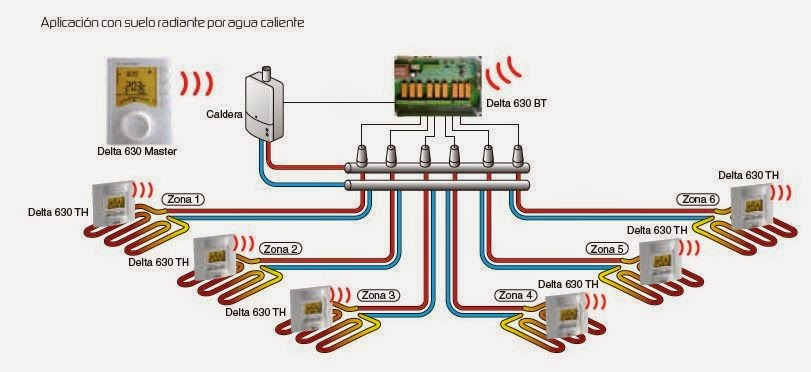
\includegraphics[width=0.9\textwidth]{seCalefaccion}
	\caption{Sistema de Calefaccion con SE.}\label{CalefaccionSE}
\end{figure}

Como podemos apreciar en la Figura \ref{CalefaccionSE} se muestran 2 sistemas embebidos, además de uno por cada zona a calentar. El primer sistema embebido, `SE1', es el que utilizará el usuario para encender la caldera y configurar la temperatura de cada zona. El SE1 se comunica con la caldera y con el `SE2'. El SE2 es el encargado de abrir o cerrar las electroválvulas que dejaran pasar el agua caliente a cada una de las zonas calentándolas. El SE2 se comunicará con cada uno de los sistemas empotrados que encontramos en cada zona para conocer la temperatura a la que están. 
Como hemos visto de esta manera podremos conseguir distintas temperaturas en cada zona dependiendo de nuestras necesidades sin necesidad de tener que subir la calefacción de todas las habitaciones de la casa o de todas las oficinas de la empresa en caso de que alguna, por ejemplo, no se esté usando en ese momento.

\section{Conexión desde otros dispositivos}\label{sec:TRConexiones}
En este apartado me gustaría hacer mención del trabajo de fin de máster que desarrolló un compañero, \cite{RPC0027}
, de esta misma universidad en el año 2018. Su TFG estaba relacionado con los sistemas empotrados. En este caso, él realizó un la conexión a Internet de una sola placa que se controlaba a través de un servidor que el gestionaba. Utilizando las interfaces propuestas en el servidor podía gestionar las luces led de la placa, tanto su color como intensidad. Me parece muy interesante la idea de poder controlar estas placas ya no solo mediante sus botones, potenciómetros, etc, sino el hecho de poder hacerlo desde un ordenador o dispositivo móvil. 
Esto es una gran idea por varias razones:
\begin{itemize}
\item En primer lugar no necesitamos de un SE que nos haga de `puente' para poder configurar las acciones de otros puesto que utilizamos un móvil u ordenador, elementos que siempre tenemos a mano. 
\item Además de esta manera conseguimos poder comunicarnos con las otras placas desde cualquier sitio y no desde donde esté físicamente ese sistema.
\end{itemize}
Roberto lo hizo, en este caso, mediante una conexión a Internet, pensando en poder comunicarnos con él aunque estemos a grandes distancias pero como se comentó en los primeros capítulos existen más formas en caso de que lo tengamos relativamente cerca, como serían bluetooth o incluso radiofrecuencias.


